%===============================================================================
%          File: ch0_introduction.tex
%        Author: Juan de Monasterio
%       Created: 15 Feb 2017
%   Description: Chapter 1: Introduction
%===============================================================================

\chapter{Introduction}
\label{cha:intro}


Chagas disease is a tropical parasitic epidemic of global reach, spread mostly across 21 Latin American countries. The World Health Organization (WHO) estimates more than six million infected people worldwide~\cite{who2016}.  Caused by the \textit{Trypanosoma cruzi} parasite, its transmission occurs mostly in the American endemic regions via the \textit{Triatoma infestans} insect family (also called ``kissing bug", and known by many local names such as ``vinchuca" in Argentina, Bolivia, Chile and Paraguay, and ``chinche" in Central America). In recent years and due to globalization and migrations, the disease has become an %health 
issue in other continents~\cite{schmunis2010chagas}, 
particularly in countries that receive Latin American immigrants such as Spain~\cite{navarro2012chagas} and the United States~\cite{hotez2013unfolding}, 
making it a global health problem.

A crucial characteristic of the infection is that it may last 10 to 30 years in an individual without being detected~\cite{rassi2012american}, which greatly complicates effective detection and treatment. About 30\% of individuals with chronic Chagas disease will develop life-threatening cardiomyopathies or gastrointestinal disorders, whereas 
the remaining individuals will never develop symptoms.
Long-term human mobility (particularly seasonal and permanent rural-urban migration) thus plays a key role in the spread of the epidemic~\cite{briceno2009chagas}. Relevant routes of transmission also include blood transfusion, congenital contagion --with an estimated 14,000 newborns infected each year in the Americas~\cite{OPS2006chagas}--,
organ transplants, 
accidental ingestion of food contaminated by \textit{Trypanosoma cruzi}, and even, in a minor scale, 
by laboratory accidents.
%Aca agregaría las otras vías de transmisión: trasplante de organos, por ingestión accidental de alimentos contaminados con T. cruzi (en italic) y en menor medida por accidentes de laboratorio.
% and worldwide treatment rates of less than 1\%.
% \begin{comment}  en el drive estan las ppt del min salud \end{comment}. 
The spatial dissemination of a congenitally transmitted disease sidesteps the available measures to control risk groups, and shows that individuals who have not been exposed to the disease vector should also be included in detection campaigns.

Mobile phone records contain information about the movements of large subsets of the population of a country, and make them very useful to understand the spreading dynamics of infectious diseases. They have been used to understand the diffusion of malaria in Kenya~\cite{wesolowski2012quantifying} and in Ivory Coast~\cite{enns2013human}, including the refining of infection models~\cite{chunara2013large}. The cited works on Ivory Coast were performed using the D4D (Data for Development) challenge datasets released in 2013. Tizzoni et al.~\cite{tizzoni2014use} compare different mobility models using theoretical approaches, available census data and models based on CDRs interactions to infer movements. They found that the models based on CDRs and mobility census data are highly correlated, illustrating their use as mobility proxies.

Mobile phone data has also been used to predict the geographic spread and timing of Dengue epidemics~\cite{wesolowski2015impact}. This analysis was performed for the country of Pakistan, which is representative of many countries on the verge of countrywide endemic dengue transmission. Other works directly study CDRs to characterize human mobility and other sociodemographic information. A complete survey of mobile traffic analysis articles may be found in~\cite{naboulsi2015mobile}, which also reviews additional studies based on the Ivory Coast dataset mentioned above. %Antenna usage is explored in \cite{sarraute2015socialevents} to automatically detect large social events, using the social graph to infer the probability of attending events.


In this work, we discuss the use of mobile phone records --also known as Call Detail Records (CDRs)-- for the analysis of mobility patterns and the detection of possible risk zones of Chagas disease in two Latin American countries. Key health expertise on the subject was provided by the \textit{Mundo Sano} Foundation.
 We generate predictions of population movements between different regions, providing a proxy for the epidemic spread. Our objective is to show that geolocalized call records are rich in social and individual information, which can be used to determine whether an individual has lived in an epidemic area. We present two case studies, in Argentina and in Mexico, using data provided by mobile phone companies from each country. %A discussion of how mobile data was processed is included. 
This is the first work that leverages mobile phone data to better understand the diffusion of the Chagas disease.




\subsection{Chagas Disease in Argentina and Mexico}

\subsection{Key Facts and Endemic Zone in Argentina}\label{endemic_zone_argentina}

For more than 50 years, vector control campaigns have been underway in Argentina as the main epidemic counter-measure. The \textit{Gran Chaco}, situated in the northern part of the country,
% is home to most of the infected triatomines
is hyperendemic for the disease~\cite{OPS2014mapa}. A map of this ecoregion is shown in Figure~\ref{fig:granchaco}.
The ecoregion's low socio-demographic conditions further support the parasite's lifecycle, where domestic interactions between humans, triatomines and animals foster the appearance of new infection cases, particularly among rural and poor areas.
% The ecoregion as of today is hyperendemic for the disease.
This region is considered as the endemic zone $E_Z$ in the analysis described in Section~\ref{methods} and Section~\ref{results}.

\begin{figure}[h!]
\centering
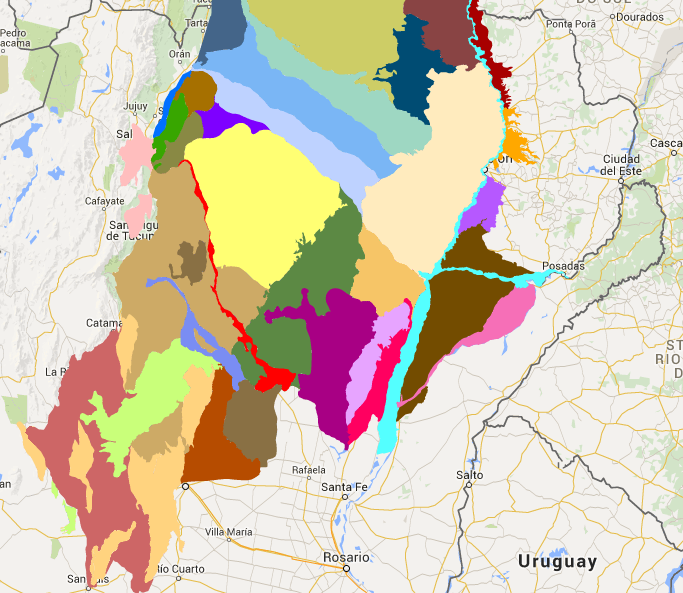
\includegraphics[width=0.75\columnwidth]{figures/Ambientes_GranChaco_TNC-Argentina/Ambientes_GranChaco_TNC-Argentina.png}
\caption{The \textit{Gran Chaco} ecoregion in South America.%
}
% \end{center}
\label{fig:granchaco}
\end{figure}


The dynamic interaction of the triatomine infested areas and the human mobility patterns create a difficult scenario to track down individuals or spots with high prevalence of infected people or transmission risk. Available methods of surveying the state of the Chagas disease in Argentina nowadays are limited to individual screenings of individuals. %The work described here is the first attempt to use mobile phone data to correlate migrations and cellphone usage to understand Chagas epidemic spatial structure. AS: WE ALREADY SAID THIS.

Recent national estimates indicate that there exist between 1.5 and 2 million individuals carrying the parasite, with more than seven million exposed. National health systems face many difficulties to effectively treat the disease. 
In Argentina, less than 1\% of infected people are diagnosed and treated 
(the same statistic holds at the world level).
% (and in Argentina, in particular, less than 1\% of infected people are treated yearly). 
Even though governmental programs have been ongoing for years now~\cite{plan_nacional_chagas}, data on the issue is scarce or hardly accessible. This presents a real obstacle to ongoing research and coordination efforts to tackle the disease in the region.


\subsection{Key Facts and Endemic Zone in Mexico} \label{endemic_zone_mexico}


\begin{figure}[h!]
\centering
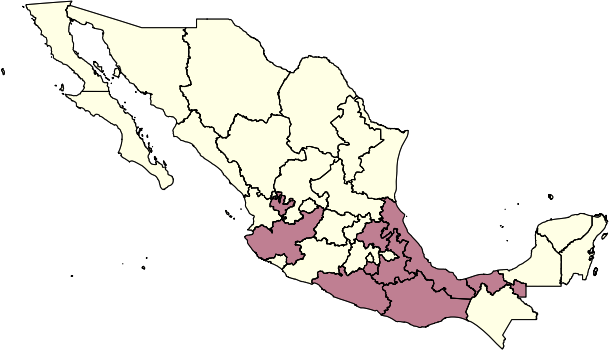
\includegraphics[width=0.75\linewidth]
{figures/Ambientes_Gran_Chaco-Mexico1/Ambientes_Gran_Chaco-Mexico1}
\caption{Endemic region $E_Z$ for Mexico.}
\label{fig:endemic_zone_mexico}
\end{figure}

In 2004, the joint work of \textit{Instituto Nacional de Cardiología ``Ignacio Chávez"} and  \textit{Instituto de Biología de la UNAM} resulted in a Chagas disease database for Mexico~\cite{cruz2006chagmex}. Reviewing positive serology in blood banks and human reported cases per state, an epidemic risk map description was produced to geographically situate the disease. Based on this data, we defined the Mexican epidemic area, selecting the states having the top 25\% prevalence rates nationwide. The resulting risk region is shown in Figure~\ref{fig:endemic_zone_mexico}. It covers most of the South region of the country and includes the states of Jalisco, Oaxaca, Veracruz, Guerrero, Morelos, Puebla, Hidalgo and Tabasco.
This region is considered as the endemic zone $E_Z$ for the Mexican case in the analysis described in Sections~\ref{methods}, \ref{results} and \ref{long_term}.




The authors of \cite{carabarin2013chagas} provide an extensive review of the 
research reports on Chagas disease in Mexico.
The review is very critical, stating that there are no effective vector control programs in Mexico;
and that the actual prevalence of the disease 
can only be estimated because no official reporting of cases is performed.
%;
%and in addition, that there is no consensus on the diagnostic methods for 
%Chagas disease in maternity wards and blood banks~\cite{carabarin2013chagas}.

According to \cite{dumonteil1999update}, 
there are a total of 18 endemic areas in Mexico, located in the southeast, and
these areas include the states of Oaxaca, Jalisco, Yucatán, Chiapas, Veracruz,
Puebla, Guerrero, Hidalgo, and Morelos, all of them with rural areas.
Chiapas, Oaxaca, Puebla, Veracruz and Yucatán are among the most affected states (where the prevalence may exceed 10\%), although cases have been reported in most areas of the country
\cite{cruz2006chagmex,dumonteil1999update}.
Despite the lack of official reports, an estimate of the number of \textit{Trypanosoma cruzi} infections by state in the country
indicates that the number of potentially
affected people in Mexico is about 5.5 million~\cite{carabarin2013chagas}.
Mexico, together with Bolivia, Colombia, and Central
America, are among the countries most affected by this 
\textit{neglected tropical disease} (NTD)~\cite{hotez2013innovation}.
The disease doesn't know about borders:
Chagas and other neglected tropical diseases present in the north of Mexico remain highly endemic in the south of Texas as well~\cite{hotez2012texas}.

In recent years there has been a focus on treating the disease with two available
medications, benznidazole or nifurtimox. A study
that explores the access to these two drugs in Mexico 
shows that less than 0.5\% of those who are infected with
the disease received treatment in Mexico in years~\cite{manne2013barriers}.


People from endemic areas of Chagas disease tend to migrate to industrialized cities of the country, mainly Mexico City, in search of jobs. 
In accordance with this movement, a report showed
that infected children under 5 year of age are frequently distributed in urban
rather than in rural areas, indicating that the disease is becoming urbanized in
Mexico~\cite{guzman2001epidemiology}.
Therefore, as in the Argentinian case, the study of long-term mobility is crucial to understand the spread of the Chagas disease in Mexico.

